\subsection{Inicialización}
En ésta fase se describirá la linea base sobre la que se desarrollará el proyecto, esto significa, definir las herramientas y dispositivos con los que se realizará el desarrollo, qué tecnologías vamos a usar y el planteamiento general del sistema.\par
\noindent
\\
\textbf{Herramientas y Tecnologías}:
	\begin{itemize}
			\item Amazon RDS
			\item Amazon S3
			\item Android 8.0 Oreo
			\item Android studio 2.19
			\item Arcore 1.5
			\item Blender 2.79
			\item Debían  9.5 “stretch”
			\item Git
			\item Git hub
			\item Java 7
	  		\item JSON
			\item Windows 10
			\item XML		
	\end{itemize}
	\noindent
\textbf{Dispositivos}:
\begin{itemize}
	\item Laptop acer, procesador Intel core i3 6ta generación, 4GB de ram, 1TB en disco duro, sistema operativo Debían  9.5 “stretch”
	\item Moto G6
	\item Moto G6 plus		
\end{itemize}
\noindent

El backend de la aplicación se encontrará sobre la infraestructura de Amazon Web Services (AWS), debido a la alta escalabilidad que proporciona. La arquitectura contendrá un cluster RDS con MySQL, cinco Lambdas, un Bucket de S3 y una API Gateway (véase Figura 3.15).\par
Cada Lambda estará enfocada a una funcionalidad principal de la aplicación:\par
\begin{itemize}
	\item\textbf{Login}.- Encargada de toda la lógica y la seguridad informática relacionada con la autenticación en la aplicación.
	\item\textbf{Registrar cuenta}.- Permitirá registrar una nueva cuenta en el sistema, misma que permitirá guardar escenarios.
	\item\textbf{Recuperar cuenta}.- En caso de que se olvide la contraseña de la cuenta, ésta Lambda contendrá la lógica para recuperar la cuenta
	\item\textbf{Guardar escenario}.- Permitirá almacenar las imágenes que sean enviadas. Estas imágenes serán almacenadas en un bucket de S3 y asociadas a un escenario. Esta información será almacenada en la base de datos de MySQL que está montada sobre el cluster de RDS.
	\item\textbf{Ver escenario}.- Ësta Lambda permitirá recuperar la información e imágenes de un escenario especificado, con el fin de poder visualizarlo desde la ubicación.
\end{itemize}
\noindent
\textbf{Arquitectura}:
La aplicación podrá comunicarse a toda la infraestructura de AWS por medio de la API Gateway, que sirve como puerta de enlace tanto para entrar como para salir de AWS. Ésta comunicación se realizará a través del protocolo HTTPS, dada la facilidad de uso que proporciona, además de la capa de seguridad SSL que ya proporciona AWS durante la comunicación con la API Gateway.
\begin{figure}[h!]
	\centering
	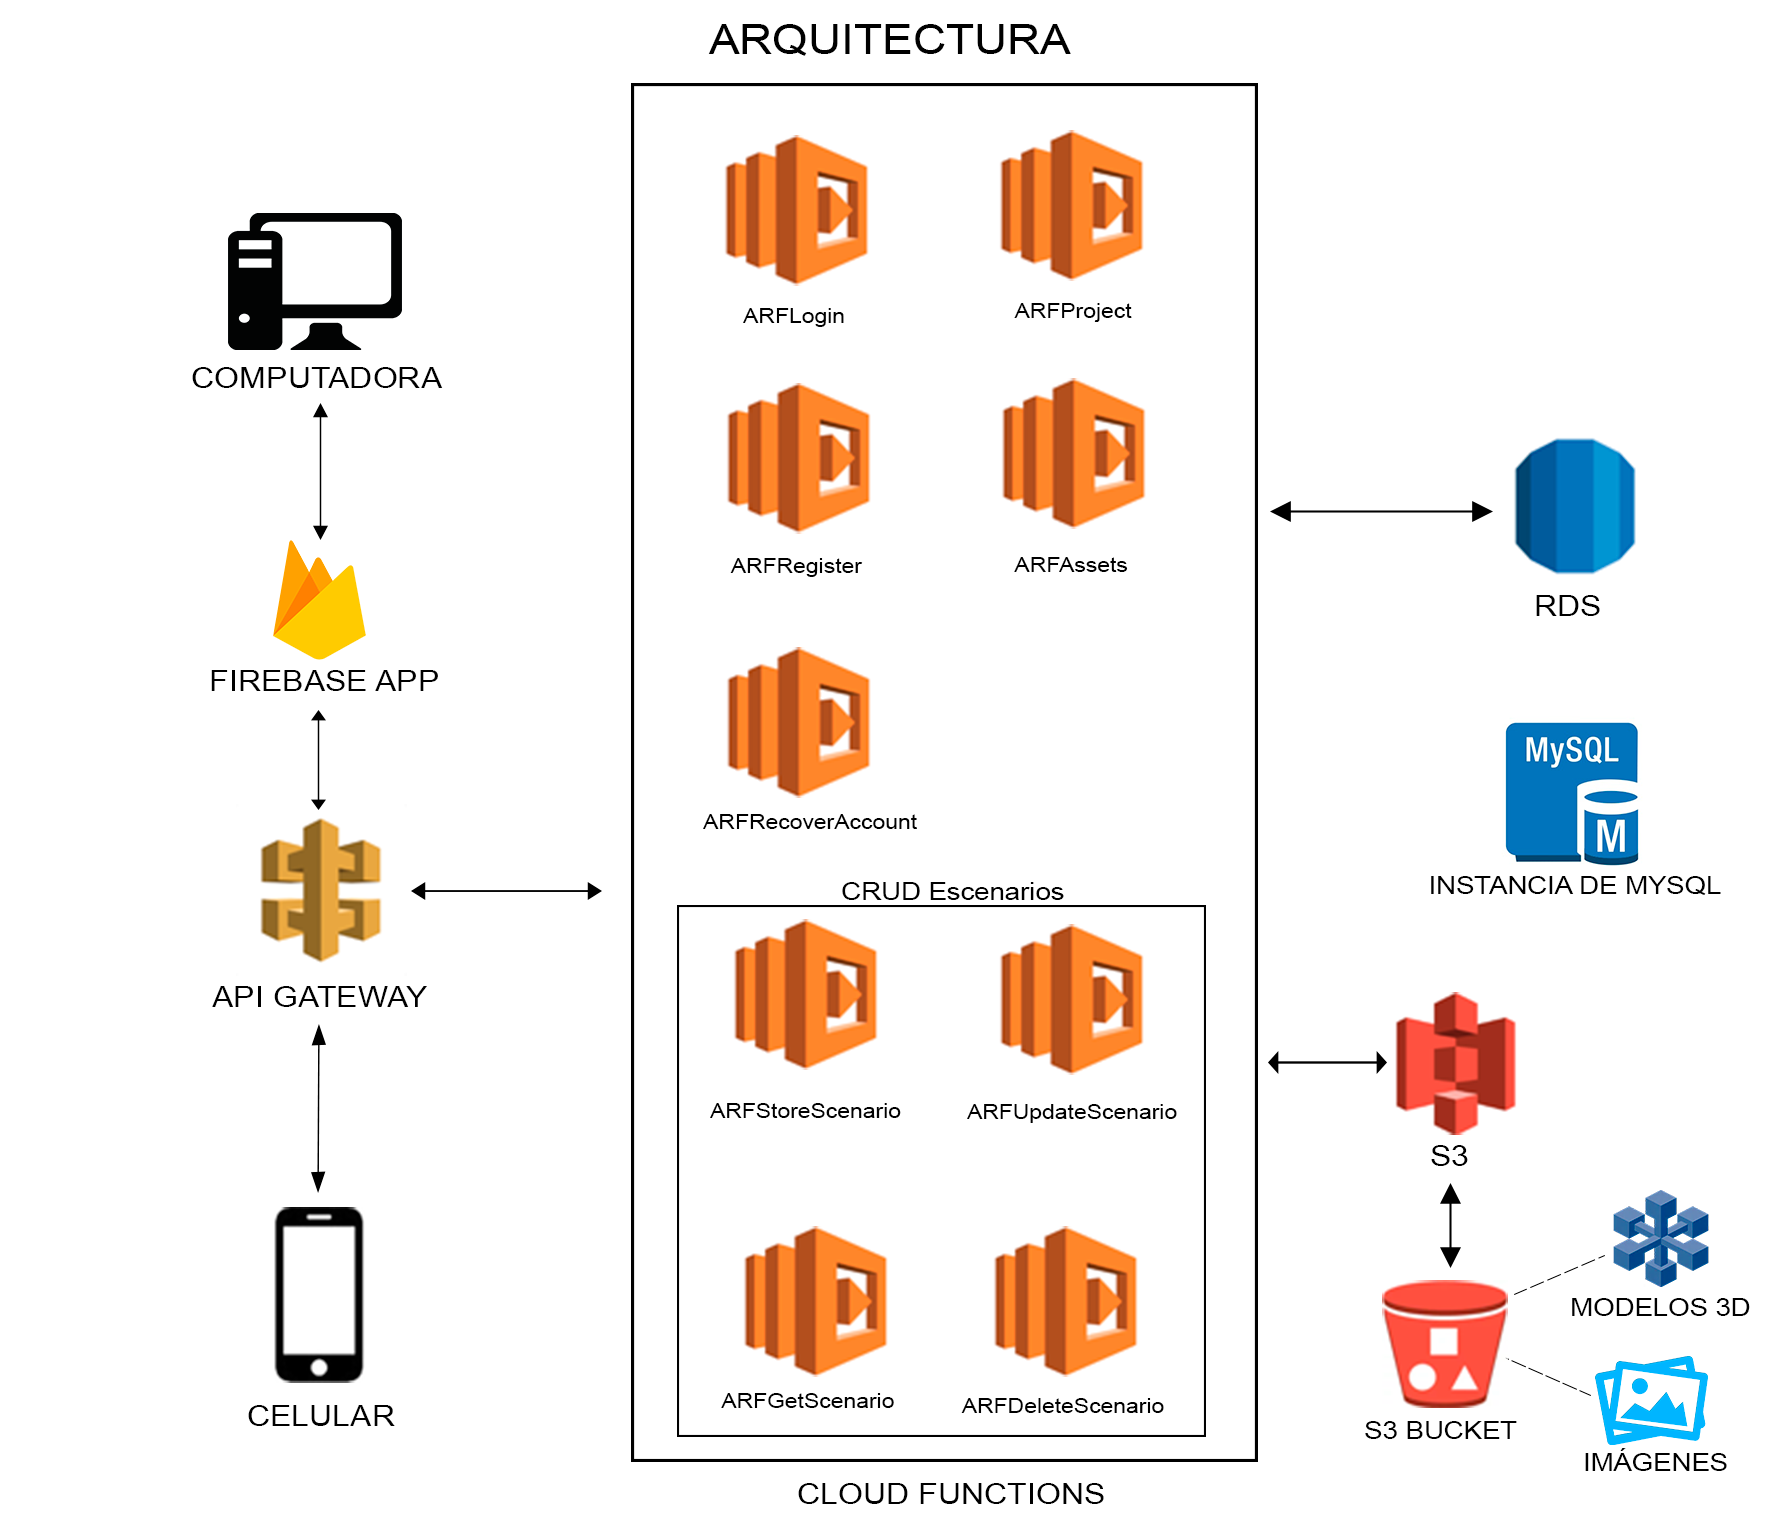
\includegraphics[width=15cm,height=15cm]{imagenes/desarrollo/arquitectura/ArchitecturaBackend.png}
	\caption{Arquitectura de Backend de ARF.}
	\label{fig:arqbackend}
\end{figure}


